\title{Artificial Life - Final Project Report: Implementing the Rosen Diagram}
\author{Ryan Spangler}
\date{\today}

\documentclass[12pt]{article}

\usepackage{commath}
\usepackage{graphicx}
\usepackage{listings}
\usepackage{amsfonts}

% python highlighting ----------
\usepackage{color}
\usepackage{listings}
\usepackage{textcomp}
\usepackage{setspace}
%\usepackage{palatino}

% \doublespacing

\setcounter{secnumdepth}{0}

\begin{document}
\maketitle

\section{Abstract}



\section{Introduction}

What is life?  This question has been asked many times, in countless forms.  It is hard to approach for many reasons: the inherent complexity of life, the dizzying variety of life's forms, the immense physical scale living things span, the tangled mess of feedback loops and reciprocities in even the simplest organisms.  The interplay of evolution and development is a riddle even the sphinx would balk at \cite{Oyama}.  

Yet as long as there is something unknown, not yet understood, people will throw themselves at the problem until the mystery has been cracked.  Just as in physics, we seek a universal solution, a succinct description or kernel that will unfold into the bewildering variety we witness.  Just as Newton's laws of gravitation provided a means for us to turn the subtle motions of the stars and celestial bodies into a single set of relationships, we long for a formalized account of biological processes, that makes the task of approaching and understanding the wide array of biological systems a tractable one.  

Beyond that, we all sense there is a unifying principle behind life.  We can *feel* it, we are instances of life ourselves.  We can immediately apprehend the living from the dead, it is obvious to discern.  It is the defining that is elusive.  

This issue of defining life is actually inseparable from the issue of making models of anything.  Modeling is how we understand the world that we can never directly experience.  A model is a substitute, a stand-in for some real world phenomenon or system we are actually interested in.  A model is useful in as much as we can perturb the model and its resulting behavior reflects the behavior of the system it was intended to model.  

In physics we build our models out of equations defining relationships between various measurable quantities.  Newton provided us with models of celestial dynamics specifically, but beyond that, and more implicitly, he provided us a general framework for defining models.  His models were such a wild success at the time people started trying to apply the same ideas to everything.  To this day, his implicit structure of defining models is still in use, still guiding the way we think about translating a natural system into a formal one.  Physics has moved on, from relativity to quantum mechanics to present day, with more and more complex models to describe the continuous revelations provided by experiment, but it is still using the same basic structure of entailment.  It is this entailment structure that has been tried, and failed, to be applied to biological systems.  Is it merely that the right model has not been found?  Or is there some deeper limitation in what kinds of models we are trying to apply to biological phenomena?

Rosen claims that there is an inherent flaw in attempting to apply the Newtonian entailment structure to biological systems \cite{Rosen}.  Specifically, Newtonian models define how one moment is translated to the next.  This is the only mode of entailment: one moment implies the next.  However, the function F which translates the previous state to the next does not change, it is static across all moments.  The states form a one-dimensional chain that can be infinitely extended by iteratively applying the universal transformation F.  It is this F that defines the system, and unearthing the F which governs the behavior of the whole universe is the main goal of physics.  

\begin{center}
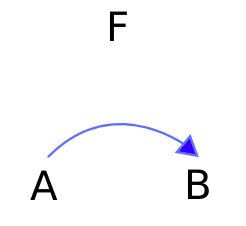
\includegraphics[scale=0.6]{newton.png}
\end{center}

In Rosen's world, F is not static.  Organisms form a closed causal loop where everything is entailed by something else within the system, including the transformation itself.  His main claim is that organisms are not modelable by chains of states governed by a static transformation.  Any transformation must itself be entailed by another transformation, which itself is generated by yet another transformation.  His full diagram is as follows:

\begin{center}
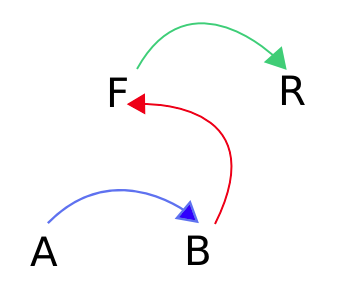
\includegraphics[scale=0.6]{rosen.png}
\end{center}

In this diagram, A entails B through F just like in Newton's model, but F itself is entailed by B from R.  R is generated from F by B.  In Rosen's terminology, F corresponds to ``metabolism'' and R to ``repair''.  A acts as the environment, an unentailed element which embodies the idea that an organism is an open system interacting with external forces beyond its membrane.  The three main functions are all entailed by other functions which are part of the system.  All the transformations act as both effector and effectee, as actor and acted-upon.  It is this diagram that I have attempted to implement for this project.

\section{Methods}

Many considerations were necessary in order to implement a system that behaves in a way representative of the diagram.  The main issue is that whatever F, B and R are, they must have the capacity to alter or influence the other elements, as well as the ability to be altered.  Specifically, there are three roles each element must play.  It must be an actor/function/transformation, taking elements from one domain into another.  Second, it must be readable, that is, a source or raw material for the transformation to work on.  Third, it must be generatable by the transformation operating on the previous element.  

What kinds of things have this structure?  A matrix can act as both a function (linear transformation at least) and data, in that it is simply a grid of numbers, so that would fulfill the requirement.  In my case though I chose to use abstract executable trees.  

A program can be thought of as a tree of instructions, with the root being the first instruction and execution taking a single path from root to leaf.  Each node is a particular operation and the branches from that node are conditional paths of execution.  So the tree only branches during conditional operations, otherwise it performs the operation of its node and continues along whatever execution path is given by its single child.  During a conditional operation the branch of execution is determined by the outcome of whatever predicate is associated with the operation.  

In this case, the operations in each node work on trees themselves, rendering each tree a program that operates on other trees.  Each tree holds iterators to both a focus and a target tree.  The focus is a node inside another tree that is currently being read: the 'A' in the diagram.   The target is indexing a node into a tree that is being altered: the 'B' in the diagram.  When the tree executes, a single execution path is chosen based on evaluating the conditions in each 'if' node as it is reached.  This execution path has operations that read from the focus tree and writes to or alters the target tree.  In the case of 'F', the conditions depend on the particular properties of the environment 'A', which can be defined according to whatever application the diagram is being implemented for.  In this way I tried to make the system general in that the environment can be defined in any way.  As long as you supply the operations which work on the environment and a function which generates values from the environment, it can correspond to whatever you want.  

For these tree operations I chose a limited set of operators: move up, move down, attach, insert, renew, and if.  The move operators are for navigating up and down the focus and target trees.  So there is a corresponding operator for moving up the focus tree as well as moving up the target tree, as well as for down.  If the iterator for that tree is already at the top when execution encounters a move up operator, nothing happens.  Likewise with move down.  

The attach operator takes the element the iterator is pointing to in the focus tree and adds it to the target node in the target tree.  Likewise with insert, but insert will actually shift the tree to add the node as a specific outlet, whereas attach will attach it to the first open outlet.  

The renew operator relates to the idea of entropy.  In the discussion of the relationship between various components in an organism, a key idea is that in the working of metabolism translating elements of the environment into energetic bonds, the actual structure of the metabolic components break down.  There is no perpetual motion machine, in order for these molecules to function they are continually expending energy and compromising their basic structure in order to carry out their tasks.  This damage to the basic components of metabolism must be offset by a process.  This process of renewal of the metabolic actors is what Rosen called the ``repair'' function, and is represented by 'R' in the diagram.  

In order to incorporate this idea of wear and renewal into this system I added in a value to each node called ``passes'', which keeps track of every time this node is visited during execution.  If the node is  a leaf and its number of passes exceeds some limit, the node is removed from the tree.  In this way the trees are progressively pruned during their operation based on how heavily the nodes are used in execution.  The renew operator then removes the wear from its target node, but at the expense of wear on itself.  This attempts to keep a balance between the proliferation of new nodes through attachments and insertions and a need to remove and wear down nodes.  However, it is a form of imposed entropy, not innate entropy as we witness in physical systems.  This is one of the greatest differences between physical systems and simulated ones, is that in physical systems entropy is an unavoidable quality of natural processes, imposed by the universe, whereas in simulated systems entropy must be inserted.  This is important because much of what organisms do can be considered in opposition to entropy, so any simulated organism by necessity is working under a contrived set of the real laws of nature which spurned its existence in the first place.  

\section{Experiments}



\section{Results}



\section{Discussion}



\section{Summary}



\bibliographystyle{plain}
\bibliography{finalreport}

\end{document}  

